\section{Patterns 5 - Model View Controller og Model View Presenter}

\subsection{Fokuspunkter}

\begin{itemize}
	\item Redegør for, hvad et software design pattern er.
	\item Redegør for Model-View-Control mønstret og dets variationer.
	\item Redegør for Model-View-Presenter mønstret og dets variationer.
\end{itemize}

\subsection{Hvad er et Software pattern?}

\derp

\subsection{Redegør for Model-View-Control mønstret og dets variationer}
MVC er et populært software pattern brugt til GUI applikationer. Ifølge Fowler er dette pattern tit misquoted. Dette skyldes at der er mange elementer i den klassiske MVC der ikke rigtig kan bruges i nutidens GUI applikationer.

\subsubsection{MVC's opbygning}
\paragraph{Model} Indeholder logik, data og states for programmet. Model kender intet til UI’et eller controller, og indeholder altså kun funktionalitet for selve business\todo{hvad er det? beskrivelse, tak} logikken. Model har et interface således at dets \textbf{state} kan tilgås eller manipuleres. Kan sende notifikationer om dets state til \textbf{observer}. Model notifier viewet, når dets state ændres\todo{en reference til observer afsnittet kunne være smart at have et sted}.

\paragraph{View} Indeholder præsentationslogik (knapper, tekstbokse, etc). Brugeren af applikationen interagerer med view, som fortæller controlleren om \textit{din} “action”. View spørger model om at få fat i data fra modellen, når modellen har annonceret en ændring i sit state.

\paragraph{Controller} Bindeleddet mellem View og Model. Controlleren indeholder logik til at finde ud af, hvad der skal ske i modellen, når brugeren trykker på noget. \textbf{Nogen gange} kan controlleren bede viewet om at ændre sig når controlleren modtager en “action” fra viewet (Enable/disable knapper/menuer).\\	

\begin{figure}[h]\todo{var den her ikke til at lukke op og skide i?}
	\centering
	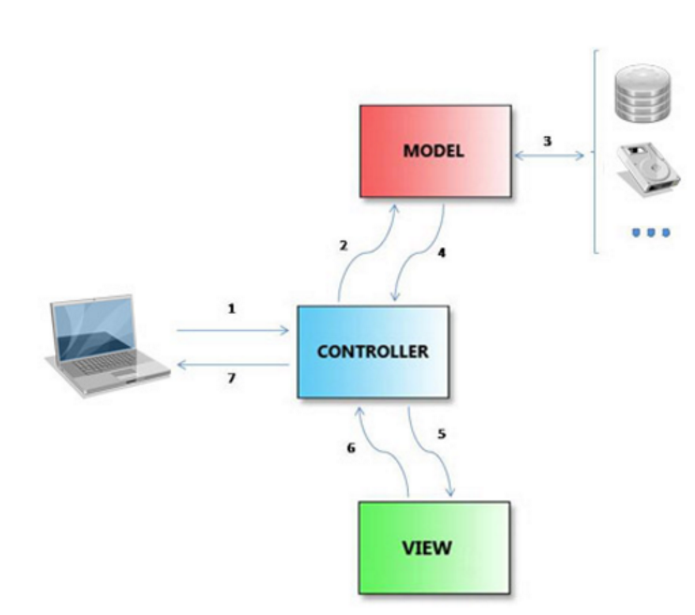
\includegraphics[width=0.7\linewidth]{figs/mvcFlow}
	\caption[Illustration af flowet i en MVC applikation]{Illustration af flowet i en MVC applikation.}
	\label{fig:mvcFlow}
\end{figure}

Brugeren trykker på en knap, som registreres af controlleren. Controlleren udfører de nødvendige handlinger på modellen, som har kontakt med evt. harddisk/database. Modellen sender svar tilbage og controlleren kalder det korrekte view, som viser dataen til brugeren.

\subsubsection{Fordele ved MVC}
\begin{itemize}
	\item Skaber høj separation mellem præsentationen (view og controller) og domænet (model).
	\begin{itemize}
		\item View og controller er separeret for at overholde SRP.
		\item forskellige Interfaces til kommunikation mellem Model-Controller og Model-View for at overholde ISP.
		\item Separation of concerns.
		\item Nemmere at teste.
		\item Nemmere at vedligeholde.
	\end{itemize}
	\item Inddeler GUI widgets i en controller som reagerer på brugerinput og view der viser modellens state. View og controller skal som regel ikke kommunikere direkte, men gennem modellen.
	\item Views (og controllere) kan observere modellen, så det er muligt for \textbf{flere widgets at opdatere}, uden nødvendigvis at behøve at kommunikere direkte. (Observer synkronisering).
\end{itemize}

\paragraph{Eksempel}
\begin{figure}[H]
	\centering
	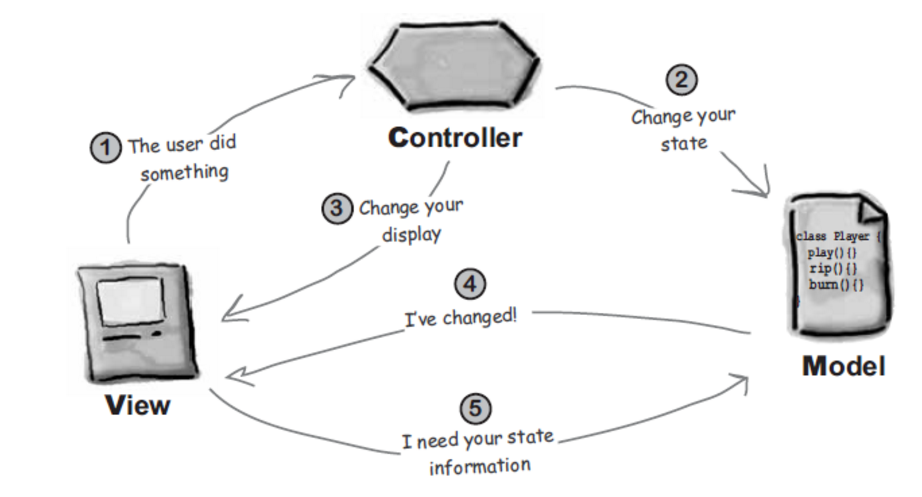
\includegraphics[width=0.8\linewidth]{figs/mvcExample}
	\caption{MVC eksemplificeret med en musik afspiller.}
	\label{fig:mvcExample}
\end{figure}

Brugeren af en media player ønsker at skifte til næste sang.

\begin{itemize}
	\item Bruger-input til view.\todo{skulle dette måske være en enumerate i stedet}
	\item Controller behandler bruger input og beder model ændre sit state herefter (kalder fx play() funktionen. Hvis det er nødvendigt kan controlleren få viewet til at ændre sig (grey out button etc.).
	\item Model annocerer at den har ændret sig.
	\item View beder om data på ændringen (fx en string i form af navnet på sangen).
	\item View opdateres.
\end{itemize}

\subsubsection{Variationer af MVC}
\todo{findes de?}

\subsection{Redegør for Model-View-Presenter mønstret og dets variationer}
MVP er en videreudviklet version af MVC, der forsøger at forene Forms and Controls med MVC \todo{hvad er FC?}.

\begin{figure}[h]
	\centering
	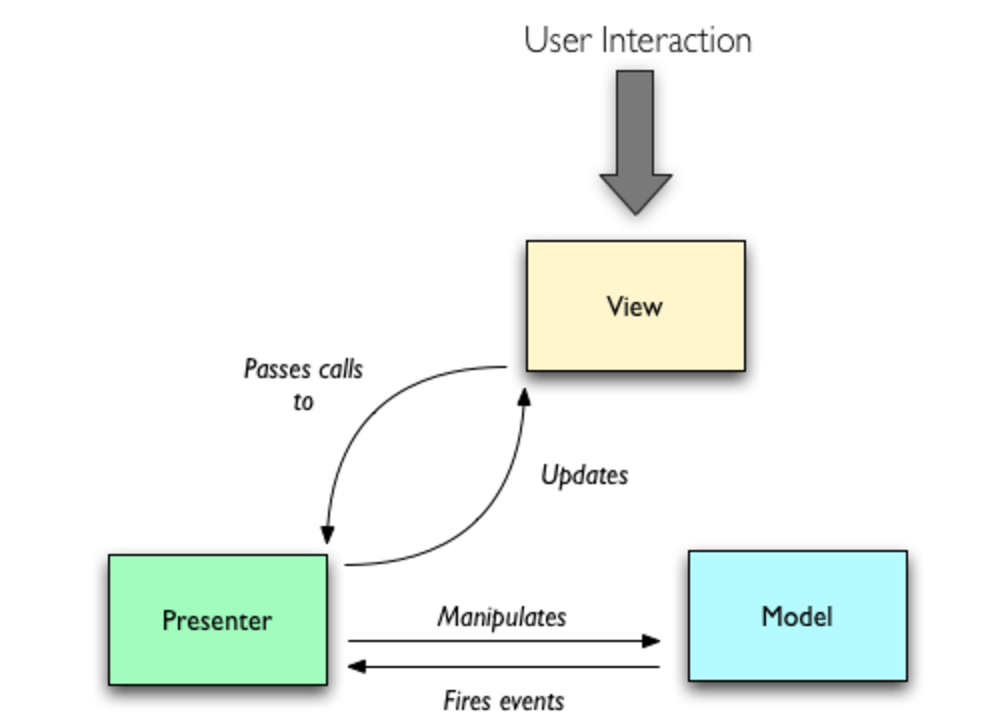
\includegraphics[width=0.7\linewidth]{figs/mvpFlow}
	\caption{Programmets flow i en MVP applikation}
	\label{fig:mvpFlow}
\end{figure}

\subsubsection{MVP's opbygning}
\paragraph{Model} Indeholder logic til at interface med programmets data.
\paragraph{View} Modtager som i MVC UI actions og kalder derved presenters funktionalitet. View indeholder typisk eventhandler og logic til at kalde presenters funktionalitet.
\paragraph{Presenter} Binder model til view (de-coupling). Har ansvaret for at opdatere view når ny data fra model. Al business logic der bruges til at behandle user inputs skrives i presenter. Presenter skal indhente data fra model, og behandle så det er klar til brug i view uden overhead.

\subsubsection{Fordele ved MVP}
\begin{itemize}
	\item I og med vi har frataget view alt dens “myndighed” og gjort den passiv. Kan vi skifte views (ændre hvordan vi ønsker at repræsentere modellen).
	\item Stærkere \textbf{separation of concerns} - view står KUN for rendering.
	\item Lettere at teste.
\end{itemize}

\subsubsection{Variationer af MVP}
Der findes to primære variationer af MVP.

\paragraph{Passive View}
Som beskrevet ovenfor.\todo{ovenfor hvor? indsæt reference.}

\paragraph{Supervising Controller}
En variation af MVP hvor viewet er mere intelligent. I denne variation har view mulighed for at kommunikere \textbf{direkte} med model og requeste data.\\

Presenter står her for at informere modellen om aktiviteter i view (der måske ændrer state). Presenter passer en reference til model så at view kan interacte med model når models state ændres. På denne måde minder MVP SC meget om MVC idet den totale de-coupling mellem view og model nu er blevet vag.
